% Acknowledgements

\pdfbookmark[1]{Acknowledgements}{Acknowledgements} % Bookmark name visible in a PDF viewer



\begin{center}
  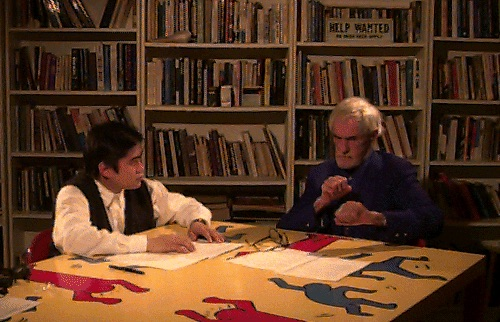
\includegraphics[width=.5\textwidth]{pictures/timleary.jpg}
  \\
  Scheming with Timothy Leary in 1995
\end{center}


\begin{flushright}{\slshape    
Question authority and think for yourself.  \\ \medskip
--- Timothy Leary}
\end{flushright}

\bigskip

%----------------------------------------------------------------------------------------

\begingroup

\let\clearpage\relax
\let\cleardoublepage\relax
\let\cleardoublepage\relax

\chapter*{Acknowledgements}

\noindent

To my late godfather Timothy Leary for ``Question Authority and Think For Yourself.''

To Jun Murai for pushing me to do this dissertation.

To my thesis advisors: Hiroya Tanaka, Rodney D. Van Meter, Keiko Okawa and Jonathan L. Zittrain for their extensive feedback, guidance and encouragement. 

To Nicholas Negroponte for the Media Lab and his mentorship.

To the late Kenichi Fukui for encouraging me to think about complex systems and the limits of reduction.

To the late John Perry Barlow for the ``Declaration of Independence of Cyberspace.''

To Hashim Sarkis for sending me in the direction of Foucault.

To Martin Nowak for his guidance on Evolutionary Dynamics.

To my colleagues at MIT and particularly at the Media Lab for continuous inspiration and my raison d'être.

To my research colleagues Karthik Dinakar, Chia Evers, Natalie Saltiel, Pratik Shah, and Andre Uhl for helping me with everything including this thesis.

To Yuka Sasaki, Stephanie Strom and Mika Tanaka for their help on helping me pull this dissertation together.

To David Weinberger for ``The final edit.''

To Sean Bonner, Danese Cooper, Ariel Ekblaw, Pieter Franken, Mizuko Ito, Mike Linksvayer, Pip Mothersill, Diane Peters, Deb Roy and Jeffrey Shapard for their feedback on various parts of the dissertation.

Finally, thanks to Kio and Mizuka for making room in our family life to work on this and for supporting me through the process.\\



\endgroup